\chapter[EPVs sobre imágenes OLCI en la SAA]{Efecto de Eventos de Partículas Veloces sobre imágenes OLCI de color del mar en la región de la Anomalía del Atlántico Sur: Detección y Remoción}
\label{ppe}

Es bien sabido que los rayos cósmicos y otras partículas masivas cargadas que se hallan atrapadas en la magnetósfera - muchas de ellas provenientes del sol - pueden eventualmente impactar sobre los dispositivos de carga acoplada (CCDs) de los sensores remotos ópticos (e.g. OLCI, MERIS) produciendo ruido eléctrico en forma de picos aislados en la señal oscura de fondo. Estos fenómenos se denominan Eventos de Partículas Veloces (EPVs), o \textit{Prompt Particle Events} en inglés, y en caso de OLCI, son el motivo de la aparición de franjas aisladas de píxeles, orientadas perpendiculares al sentido de barrido donde los valores de radiancia medidos resultan anómalamente altos o bajos con respecto a los valores de píxeles próximos. La magnitud y frecuencia de dichas franjas es evidentemente más alta en la región de la Anomalía Magnética del Atlántico Sur (\textit{South Atlantic Anomaly}, SAA), que también abarca la región central de Sudamérica, incluyendo al Río de la Plata. En esta región, la contaminación de las imágenes OLCI de radiancia a TOA tiene un impacto significativo sobre la reflectancia del agua y sobre el cómputo de productos biogeofísicos derivados, provenientes de píxeles que se hallan dentro de dichas franjas. Esto significa que para poder brindar valores confiables de dichos productos satelitales es imprescindible que dichas franjas sean detectadas y removidas de las imágenes nivel 1B (L1B) de OLCI.

Si bien la motivación original de la presente tesis es la implementación de correcciones atmosféricas sobre aguas turbias, el hecho de que el Río de la Plata es simultáneamente nuestra principal región de interés y el único cuerpo de agua turbia de gran extensión que se halla inmerso dentro del área de influencia de la Anomalía Magnética del Atlántico Sur, nos condujo, tanto por necesidad como por exploración, a la tarea imprescendible de implementar un algoritmo de detección y remoción de EPVs sobre imágenes OLCI en la región del Atlántico Sur.

El algoritmo que se desarrolló es globalmente aplicable a imágenes OLCI (y MERIS, aunque no fue testeado en dichas imágenes) sobre cualquier cuerpo de agua, y está basado en un filtro espacial móvil con un núcleo de 5 px $\times$ 1 px orientado en sentido del barrido de la imagen. El algoritmo se aplica sobre el conjunto espectral total de radiancias a TOA de OLCI. Su desempeño fue evaluado tanto visualmente (dado que, por obvias razones, es imposible una validación \textit{in situ}) como mediante comparación con resultados teóricos preexistentes. Los resultados indican que las imágenes sobre la región de la SAA contienen 27.8 veces más píxeles contaminados por EPVs que las correspondientes a regiones por fuera de la SAA y que las bandas más afectadas son las de 400 y 1016 nm, donde la fracción de píxeles detectados como contaminados por EPVs sobre la SAA alcanzó el 0.14\% y 0.26\%, respectivamente.

$\quad$

\noindent
El contenido del presente capítulo se halla publicado en:

$\quad$

\noindent
GOSSN, J.I. (2018) Effect of Prompt Particle Events on OLCI Ocean Color Imagery in the South Atlantic Anomaly: Detection and Removal. IEEE GEOSCIENCE AND REMOTE SENSING LETTERS.: IEEE-INST ELECTRICAL ELECTRONICS ENGINEERS INC. vol. 16, no. 2, pp. 163-167. doi: 10.1109/LGRS.2018.2872172, \cite{gossn2018}

\section{Introducción}
\label{ppe:s:introduction}

    La Anomalía Magnética del Atlántico Sur (\textit{South Atlantic Anomaly}, SAA) es una alteración topológica del campo magnético terrestre que impacta directamente en la altura del cinturón de radiación en la región de Sudamérica central y el Atlántico Sur adyacente a las costas de Brasil, Uruguay y Argentina central. El cinturón de radiación es una región de la alta atmósfera terrestre donde existe un flujo de partículas cargadas cuyas trayectorias son espirales alrededor de las líneas de campo magnético tales que su radio de rotación tiende a encerrar un flujo magnético constante \cite{sturrock1994}. El campo magnético terrestre no es un dipolo magnético geodésicamente centrado, sino que puede ser \textit{aproximadamente} representado por un dipolo desplazado levemente hacia el norte del centro geodésico de la Tierra, de forma tal de que la región de la Anomalía del Atlántico Sur se halla más alejada que el resto de la superficie terrestre. Esto significa que cada partícula cargada de trayectoria espiralada alrededor de las líneas de campo va a desplazarse hacia altitudes menores de forma tal de encerrar un flujo magnético constante al aproximarse a la región de la SAA. En otros términos, el cinturón de radiación que rodea a la Tierra, definido precisamente por la presencia de dichos electrones y protones de altas energías (comprendidas en el rango de 0.001-100 MeV \cite{cravens1997}), es usualmente encontrado (dentro de la SAA) en altitudes similares a las de satélites terrestres de órbitas bajas \cite{badhwar1999} (\textit{Low Earth Orbit}, LEO), como por ejemplo el cuarteto de plataformas de Sentinel-3/OLCI (de las cuales, hasta el presente año 2020 sólo dos están en órbita, a saber, A \& B) y EnviSat/MERIS, cuyas altitudes son 814.15 $km$ \cite{nieke2004} y 782 $km$ \cite{eumetsat}, respectivamente. 
    Al colisionar dichas partículas con los CCDs de los sensores con órbitas tipo LEO se produce un fenómeno llamado EPV (Evento de Partícula Veloz), que consta de ruido eléctrico en forma de picos aislados en la señal oscura de fondo. Particularmente, los diseños técnicos específicos de los dispositivos de carga acoplada (CCDs) de OLCI y MERIS (exhaustivamente descritos en D' Amico et al. 2015, \cite{damico2015}), hacen que estos estén fuertemente afectados por los EPVs de manera global, pero particularmente cuando están orbitando alrededor de la SAA.
    
    En caso de producirse un EPV, una serie de múltiples picos aparecen en la señal de fondo, dado que su intensidad es suficientemente baja en comparación con el ruido provocado por las partículas energéticas que impactan en los CCDs, resultando en radiancias a TOA anómalamente bajas/altas. Debido al hecho de que sendas dimensiones espaciales de los CCDs se corresponden con la dirección de barrido y el rango espectral abarcado por el conjunto de bandas OLCI (pues es un sensor tipo \textit{pushbroom}, Figura \ref{ppe:CCD_OLCI}), respectivamente\footnote{cada píxel del CCD tiene un tamaño de 22.5 $\mu m$, correspondiente a aproximadamente una extensión \textit{across-track}/espectral de 300 m $\times$ 1.25 nm.}, y dado que cada EPV puede afectar varios elementos adyacentes, es esperable que los errores inducidos por los EPVs se visualicen como franjas ortogonales a la dirección de barrido (\textit{across-track}) y a lo largo de varias bandas dentro de los archivos de nivel L1B, aunque tanto la extensión \textit{across-track} como la espectral afectada resulta incierta y dependerá de la energía, la orientación de impacto y la naturaleza física de la partícula, \cite{damico2015}.
    
    \begin{figure}
    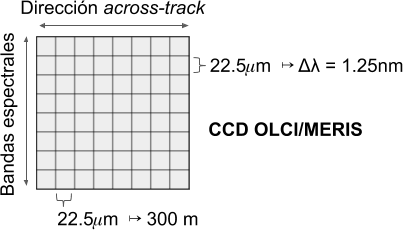
\includegraphics[width=0.4\textwidth]{ppe/figures/CCD_OLCI.png}
    \caption[Representación de un dispositivo de carga acoplada (CCD) de OLCI o MERIS.]{Representación de un dispositivo de carga acoplada (CCD) de OLCI o MERIS. Cada dimensión del CCD se corresponde al rango espectral barrido por las bandas del sensor y a la dirección \textit{across-track} o de traverso-barrido.}
    \label{ppe:CCD_OLCI}
    \end{figure}
    
    El efecto de los EPVs sobre las radiancias a TOA ha sido previamente estudiado sobre imágenes MERIS, así como el efecto que los mismos tienen sobre los productos derivados de las mismas. Un ejemplo es el caso del producto \textit{Índice de Máxima Clorofila} (\textit{Maximum Chlorophyll Index}, MCI), cuya definición es \cite{gower2008}:
    
    \begin{equation}
    MCI =  -0.6164.L^{TOA}_{681} + L^{TOA}_{709} -0.3836.L^{TOA}_{754}
    \label{ppe:eq:mci}
    \end{equation}
    
    \noindent
    donde $L^{TOA}_{XXX}$ es la radiancia a TOA en la banda espectral centrada en $XXX$ nm. Se encontró en la SAA, que los mapas de MCI presentan una alta densidad de píxeles aislados con valores anómalos. Dicho fenómeno ha sido analizado y vinculado a la presencia de EPVs \cite{gower2008}. El presente estudio está enfocado en presentar un algoritmo simple diseñado para detectar y remover valores anómalos de radiancias a TOA (\textit{i.e.} presentes al nivel L1B) inducidos por EPVs, para los sensores OLCI y MERIS. El método propuesto está basado en un núcleo móvil píxel a píxel de tamaño 5 px $\times$ 1 px alineado con la dirección de barrido (\textit{along-track}), a ser aplicado sobre cada banda. Dicho método fue testeado e implementado exitosamente en imágenes OLCI. El desempeño del mismo fue evaluado visualmente y mediante la comparación con predicciones preexistentes \cite{damico2015} de la fracción de píxeles contaminados y su error asociado sobre la radiancia a TOA. A su vez, por transitividad, la implementación de dicho mecanismo de remoción de EPVs sobre datos de nivel L1B permitirá la reducción de valores erróneos en productos derivados de radiancias a TOA, tales como el MCI, las reflectancias superficiales, entre muchos otros.

\section{Datos satelitales}
\label{ppe:s:satelitales}

    Un total de 18 imágenes nivel L1B fueron utilizadas para comparar tanto la cantidad de píxeles contaminados como la intensidad del error inducido por EPVs. Para ello fueron seleccionadas subregiones de $1\degree\times1\degree$ de imágenes en ausencia total de nubosidad y tierra. La mitad de dicho conjunto correspondió a zonas contenidas en la SAA y la otra mitad a zonas del noroeste del mar de Australia. Dichos subconjuntos son identificados como SAA y AUS, respectivamente, y sus ubicaciones geográficas aproximadas marcadas en la Fig. \ref{ppe:ppeMagnetic} en rojo y azul, respectivamente.
    
    Los datos fueron descargados del sistema de adquisición de datos en línea Copernicus (\textit{Copernicus Online Data Access}, CODA) y corresponden a la línea de procesamiento base 2.23, es decir, el primer reprocesamiento global sobre imágenes OLCI \cite{eumetsat}. 
    La subregión seleccionada de la SAA corresponde al Océano Atlántico adyacente a las costas de Argentina, Brasil y Uruguay, incluyendo las aguas extremadamente turbias del estuario del Río de la Plata, entre Argentina y Uruguay. En esta región seleccionada, la intensidad del campo geomagnético a la altura de órbita del satélite es cercana al mínimo ($\sim 19000 \, nT$ a 614 km s.n.m.). Por otro lado, la región llamada aquí AUS corresponde al Océano Índico adyacente a la costa noroeste australiana, donde coexisten una alta intensidad de campo geomagnético y una baja cobertura nubosa promedio \cite{esacloud}.
    
    \begin{figure}
    \centering
    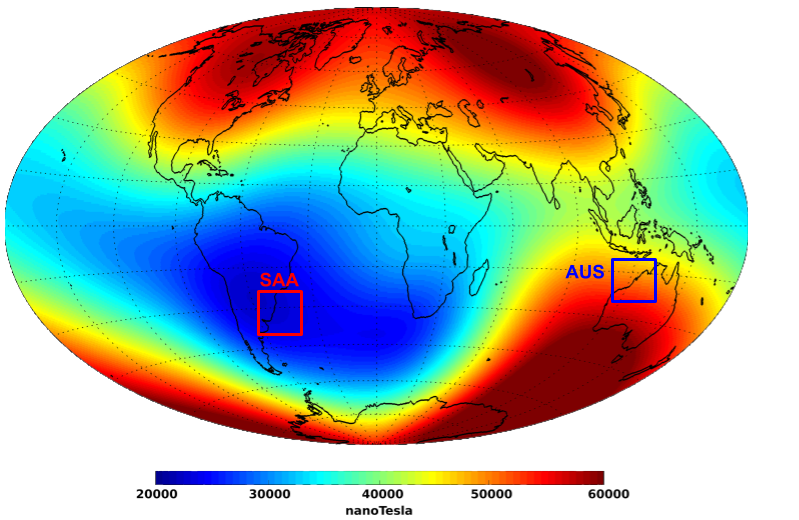
\includegraphics[width=\textwidth]{ppe/figures/ppeMagnetic.png}
    \caption[Intensidad total del campo magnético terrestre a la altura de la superficie terrestre.]{Intensidad total del campo magnético terrestre a la altura de la superficie de la Tierra, adquirida por la Constelación Swarm entre 01-ENE-2014 y 30-JUN-2014. Las cajas roja y azul indican las regiones a comparar en este trabajo: el Océano Atlántico adyacente a las costas de Argentina, Uruguay y Brasil (dentro de la Anomalía Magnética del Atlántico Sur, SAA), y el Océano Índico adyacente al noroeste de la costa australiana (AUS), respectivamente.}
    \label{ppe:ppeMagnetic}
    \end{figure}
    
    \begin{table}
    \caption[Tiempos de adquisición de las imágenes utilizadas para identificar el efecto de la SAA sobre la frecuencia e intesidad de los EPVs.]{Tiempos de adquisición de las imágenes utilizadas para identificar el efecto de la SAA sobre la frecuencia e intesidad de los EPVs. Corresponden a las regiones SAA y AUS, marcadas en la Fig. \ref{ppe:ppeMagnetic}.}
    \centering
    %% \tablesize{} %% You can specify the fontsize here, e.g.  \tablesize{\footnotesize}. If commented out \small will be used.
    \begin{tabular}{|l|l|l|}
    \hline
    \textbf{Nro. imagen} & \textbf{SAA} & \textbf{AUS}\\
    \hline
    1 & 2017-10-07T13:10:14Z & 2017-10-13T02:02:12Z \\
    \hline
    2 & 2017-10-15T13:02:45Z & 2017-10-14T01:36:01Z \\
    \hline
    3 & 2017-10-16T12:36:34Z & 2017-10-18T01:32:17Z \\
    \hline
    4 & 2017-10-19T12:59:00Z & 2017-10-25T01:50:59Z \\
    \hline
    5 & 2017-10-30T13:13:58Z & 2017-10-26T01:24:48Z \\
    \hline
    6 & 2017-10-31T12:47:47Z & 2017-10-29T01:47:15Z \\
    \hline
    7 & 2017-12-24T12:47:47Z & 2017-11-17T01:54:43Z \\
    \hline
    8 & 2018-01-04T13:02:45Z & 2017-11-29T01:43:30Z \\
    \hline
    9 & 2018-01-08T12:59:01Z & 2017-11-30T01:17:19Z \\
    \hline
    \end{tabular}
    \label{tab:img}
    \end{table}
    
    El desarrollo, sondeo e implementación del algoritmo fue realizado sobre productos OLCI nivel L1B, es decir, sobre matrices de radiancias a TOA que siguen la geometría de los píxeles de los CCDs. Esto significa que las filas y columnas de las radiancias a TOA corresponen a las direcciones de barrido (\textit{along-track}) y traverso-barrido (\textit{across-track}), respectivamente.
    
    \begin{figure*}
    \centering
    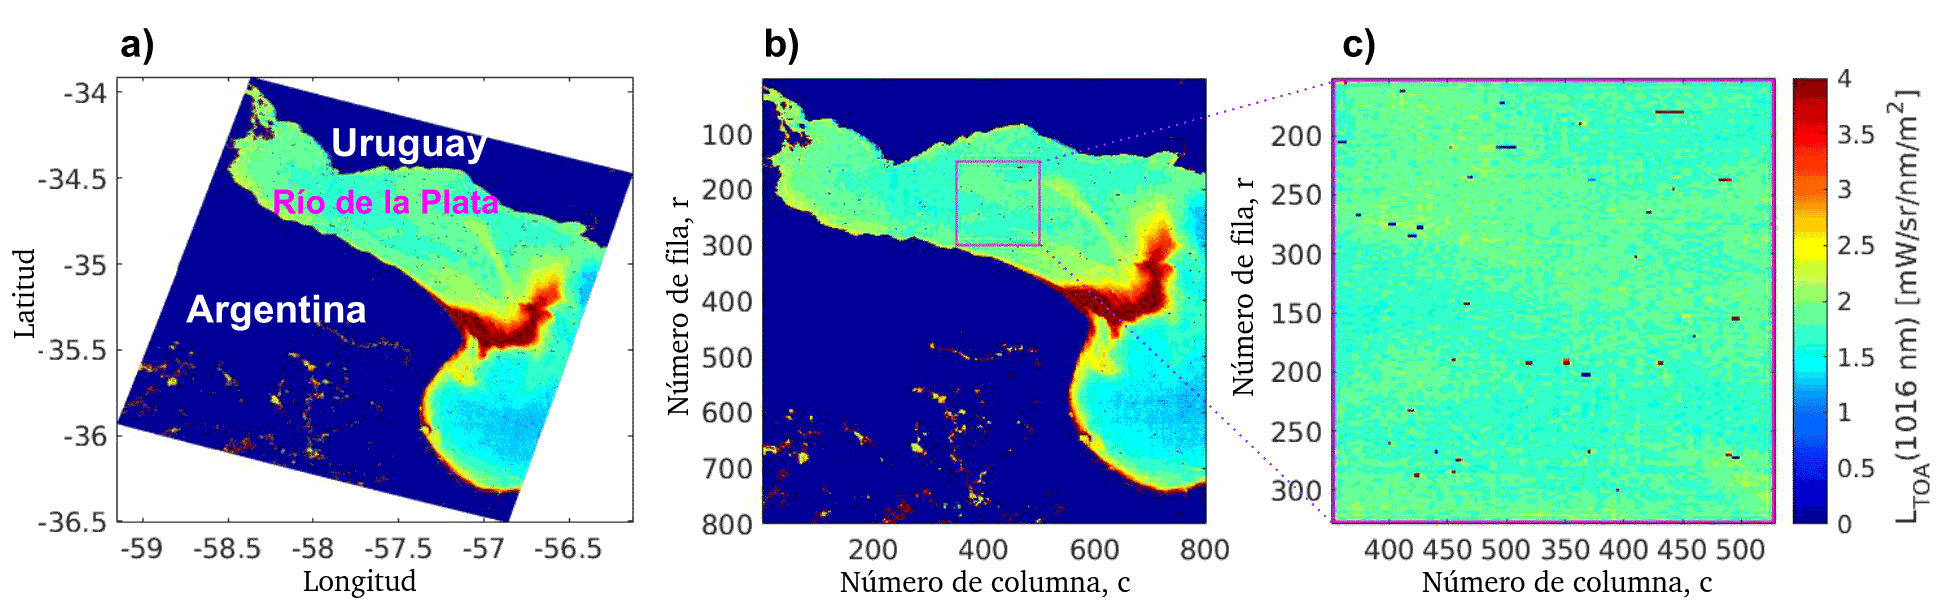
\includegraphics[width=\textwidth]{ppe/figures/ppeRdP}
    \caption[Radiancia a tope de la atmósfera a 1016 nm tomada por OLCI sobre el RdP (SAA) afectada por la presencia de EPVs.]{Radiancia a tope de la atmósfera a 1016 nm tomada por OLCI sobre el Río de la Plata dentro de la región SAA (fecha de adquisición: 2017-09-18T13:02:45Z), donde la presencia de EPVs se observa como rayas de píxeles aisladas con un brillo extremadamente alto o bajo. a) Proyección Plate-Carrée, b) Geometría de fila-columna (como en los datos nivel L1B), donde las franjas de píxeles contaminadas con EPVs están en sentido traverso-barrido, y c) ampliación en una subregión más pequeña para visualizar mejor los píxeles contaminados.}
    \label{ppe:ppeRdP}
    \end{figure*}

    Se consideraron dos razones complementarias para implementar el algoritmo en esta geometría: i) el efecto inducido por las EPVs está orientado perpendicular al barrido, y ii) los potenciales artefactos de límite de cámara están orientados a lo largo del barrido, junto con otros artefactos como el ruido de patrón fijo (\textit{Fixed Pattern Noise}) \cite{damico2015}. Esto significa que en esta geometría los EPVs son fácilmente identificables como franjas transversales y a su vez ortogonales con respecto a los eventuales efectos de cámara orientados \textit{along-track}.

\section{Algoritmo de detección y remoción}
\label{ppe:s:algo}

    La detección de píxeles contaminados con EPVs en imágenes L1B se aplicó sobre cada banda OLCI por separado, píxel a píxel. El esquema puede resumirse en los siguientes pasos (ver Fig. \ref{ppe:ppeAlgo}):
    
    \begin{enumerate}
        \item Para un dado píxel, ubicado en $(r,c)$ (i.e. en la fila $r$ y la columna $c$), un núcleo de 5 px $\times$ 1 px orientado en la dirección de barrido es considerado contemplando al propio píxel y al grupo de píxeles vecinos dentro del barrido $(r',c)$, siendo $r'={r-2,r-1,r+1,r+2}$.
        
        \item Se calculan la mediana y la desviación absoluta mediana (\textit{Median Absolute Deviation}, MAD) de las radiaciones TOA en los píxeles en $(r',c)$ de $L^{TOA}_{r',c}$ ($ mdn(L^{TOA}_{r', c}) $ y $ MAD(L^{TOA}_{r',c})$, resp.). La desviación absoluta mediana se define como:
    
        \begin{equation}
            MAD(L^{TOA}_{r',c}) := mdn( | L^{TOA}_{r',c} - mdn(L^{TOA}_{r',c}) | )
            \label{ppe:eq:mad}
        \end{equation}

        \noindent
        siendo $mdn(\cdot)$ la mediana y $|\cdot|$ el módulo.

        \item Si el valor de radiancia TOA en $(r,c)$ difiere de la mediana en más de diez veces la desviación absoluta mediana y también difiere en más de un umbral mínimo de 0.7 $mW/nm/sr/m^{2}$, entonces se establece una alerta de EPV en dicho píxel. Matemáticamente, la condición se puede expresar de la siguiente manera:

        \begin{equation}
            |L^{TOA}_{r,c} - mdn(L^{TOA}_{r',c}) | > \\ max\{10.MAD(L^{TOA}_{r',c}) ; 0.7\}
            \label{ppe:eq:ppr}
        \end{equation}
    
        \item Si la alerta de EPV está activada, el valor de radiancia TOA afectado en el píxel $(r,c)$ se reemplaza por la mediana del conjunto $(r',c)$, es decir, $L^{TOA}_{r,c}\rightarrow mdn(L^{TOA}_{r',c})$. El indicador EPV podría propagarse a los datos del Nivel 2 para notificar a los usuarios que se ha utilizado un valor de reemplazo.
    
    \end{enumerate}

    \begin{figure}
    \centering
    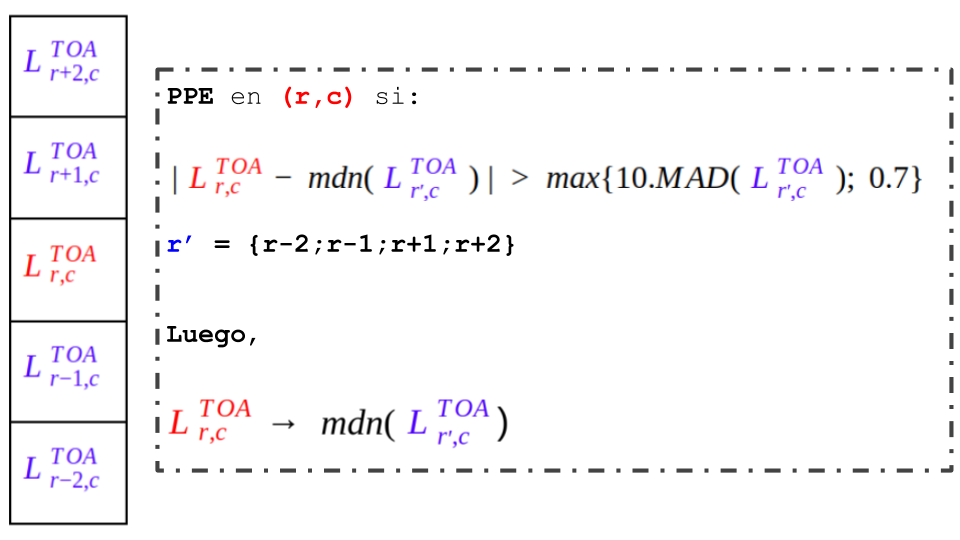
\includegraphics[width=0.75\textwidth]{ppe/figures/ppeAlgo}
    \caption[Esquema que describe el algoritmo de detección de EPVs para un píxel determinado.]{Esquema que describe el algoritmo de detección de EPVs para un píxel determinado ubicado en $(r,c)$, basado en la comparación de su radiancia a TOA con las radiancias en sus cuatro vecinos más cercanos en el sentido \textit{along-track} (llamados aquí $(r', c)$).}
    \label{ppe:ppeAlgo}
    \end{figure}

    El algoritmo contempla a los cuatro vecinos más cercanos en dirección del barrido en lugar de dos porque las franjas transversales producidas por la contaminación del EPV pueden tomar más de una fila en casos excepcionales (hasta tres filas). También utiliza la mediana y el MAD como medidas de valor central y dispersión dado que son estadísticos más robustos con respecto a la presencia de anomalías en comparación con los estadísticos habituales, como la media y la desviación estándar. Estas anomalías pueden ser producidas, en los casos de alta contaminación de EPVs, por otros EPVs que afectan los píxeles $(r',c)$. Esto ocurre sólo en casos excepcionales dentro del SAA y en bandas altamente contaminadas (como 400 nm y 1016 nm).
    El factor 10 aplicado al término MAD se determinó a partir de la inspección visual de escenas nubladas donde, dados factores menores que 10, las nubes pequeñas se detectaron incorrectamente como EPVs.
    %%
    Finalmente, el umbral mínimo de radiancia de 0.7 $mW/nm/sr/m^{2}$ se estableció para evitar falsos indicadores de EPVs donde la variabilidad en los píxeles del conjunto $(r',c)$, cuantificada a través de $MAD(L^{TOA}_{r',c})$, es anómalamente pequeña. A su vez, está asociado con la naturaleza del error inducido por el EPV en la radiancia a TOA: D' Amico et al. 2015 \cite{damico2015} predijeron que, dado que un píxel está contaminado por un EPV, se espera que la función de densidad de probabilidad sobre el error absoluto de radiancia TOA siga una ley de decaimiento exponencial simple con una escala característica de 1 y un paso inicial de 0.81 $mW/nm/sr/m^{2}$ (esto significa una probabilidad nula de ser menor que 0.81 $mW/nm/sr/m^{2}$, cf. D' Amico et al. 2015, Fig. 6f). El umbral más pequeño de 0.7 $mW/nm/sr/m^{2}$ se estableció para tener en cuenta casos excepcionales en los que el error inducido por EPVs es ligeramente menor que 0.81 $mW/nm/sr/m^{2}$.
    
    Debe mencionarse que, en general, las nubes pequeñas, las islas o cualquier otra fuente natural de variabilidad no siguen en general la orientación espacial específica de los EPVs en la dirección de barrido, pero excepcionalmente podrían afectar líneas solitarias.
    En los casos excepcionales de islas pequeñas, éstas deberían ser detectadas por máscaras terrestres preexistentes, y no está al alcance de este algoritmo detectarlas. El término $10 MAD(L^{TOA}_{r',c})$ generalmente evita que se detecten nubes pequeñas como EPV, pero también el enmascaramiento de nubes preexistente no debería confundir nubes con EPVs dado que las nubes son espectralmente casi blancas, mientras que los EPVs en general no son blancos, sino que afectan a las bandas cercanas a la región del CCD impactada por el EPV.
    En los casos de costas, plumas de turbidez u otras fuentes de variabilidad natural, las variaciones espaciales observadas son más suaves que las producidas por EPVs o bien la diferencia en los valores de radiancia dentro de cada núcleo en dirección del barrido no es lo suficientemente alta como para ser detectada como EPV.

\section{Resultados y discusión}
\label{ppe:s:resultados}

    La Figura \ref{ppe:ppeAUSSAA} muestra un ejemplo de cómo funciona la eliminación de EPVs para dos escenas, una dentro del la región SAA (2017-10-19T12:59:00Z) y otra dentro de la región AUS (2017-10-25T01:50:59Z) (las regiones SAA y AUS se muestran en la Fig. \ref{ppe:ppeMagnetic}). Se eligió la banda de 1016 nm (Oa\_21) para ilustrar la eliminación de EPVs ya que es la más afectada de las 21 bandas de OLCI (ver Fig. \ref{ppe:ppeBands}). Esto muestra cómo los EPVs se producen con mayor frecuencia en la región de la Anomalía del Atlántico Sur en comparación con otros sitios donde la intensidad del campo magnético es mayor a la altura de órbita de OLCI.
    
    \begin{figure}
    \centering
    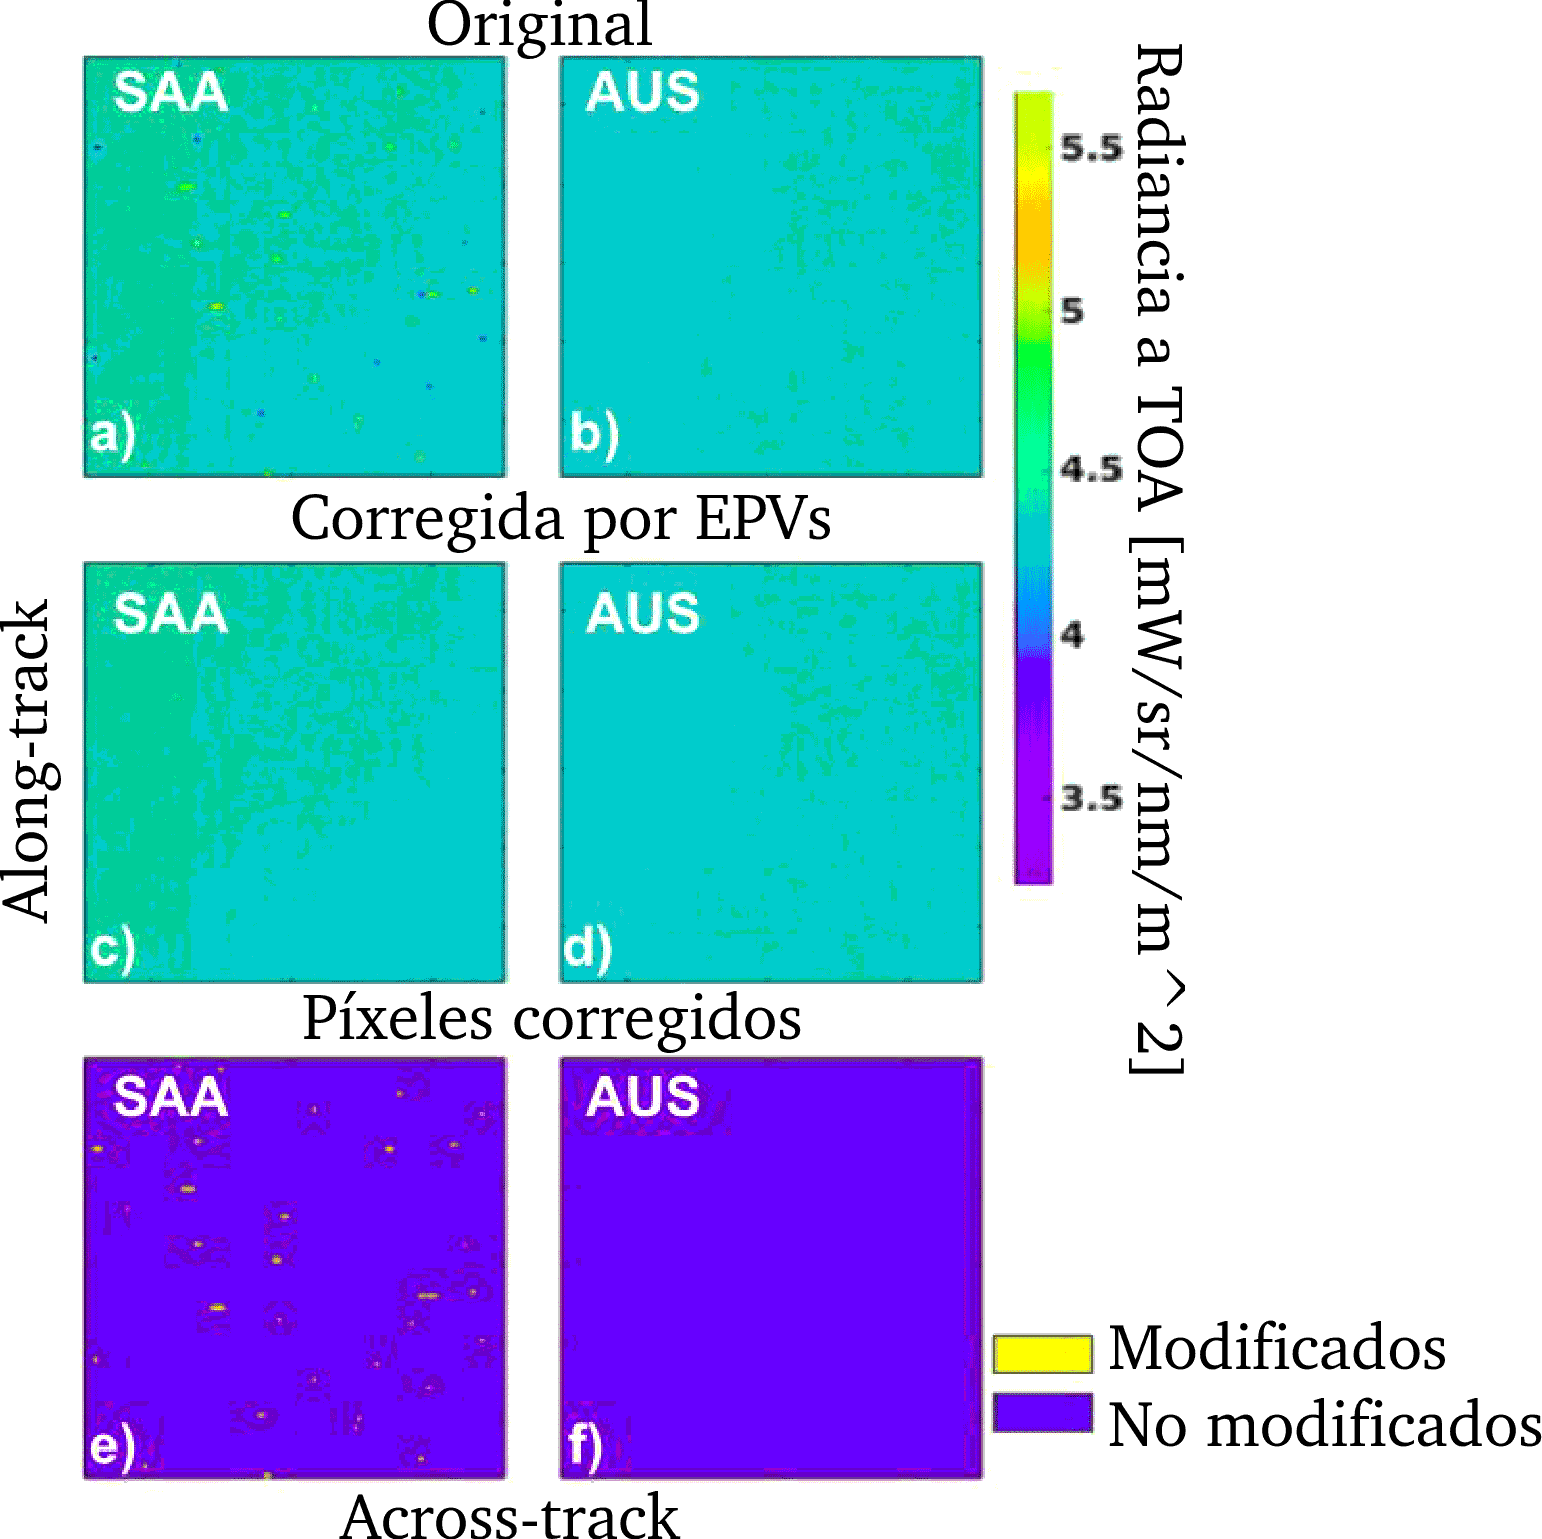
\includegraphics[width=0.7\textwidth]{ppe/figures/ppeAUSSAA}
    \caption[Efecto del esquema de eliminación de EPVs sobre la radiancia de TOA a 1016 nm para las regiones SAA y AUS.]{Efecto del esquema de eliminación de EPVs sobre la radiancia de TOA a 1016 nm para las regiones SAA (izquierda) y AUS (derecha). Los recuadros a) y b) muestran las radiancias a TOA en 1016 nm, c) y d) las mismas radiancias pero corregidas por EPVs (donde los píxeles marcados se corrigieron como se describe en \S \ref{ppe:s:algo}, Fig. \ref{ppe:ppeAlgo}), y en e) y f) los píxeles marcados con EPVs se muestran en amarillo.}
    \label{ppe:ppeAUSSAA}
    \end{figure}
    
    La Figura \ref{ppe:ppeBands} muestra los porcentajes de píxeles marcados con EPVs dentro de las regiones de estudio seleccionadas SAA y AUS para cada una de las 21 bandas en OLCI. Los dos conjuntos se compusieron de 9 imágenes de $1 \degree \times 1 \degree$ en ausencia de tierra y nubes desde el período septiembre de 2017 hasta enero de 2018. Las fracciones informadas se calculan como el número total de píxeles marcados con EPVs sobre el total de píxeles de los 9 subconjuntos considerados para cada región. Es claramente observable en la Fig. \ref{ppe:ppeBands} cómo la región SAA se ve más afectada por los eventos de EPVs que AUS, la cual se halla más \textit{protegida magnéticamente}, lo que significa que los EPVs son altamente improbables en comparación. Un porcentaje mayor de píxeles marcados con EPVs se observa para SAA en las bandas de 400 nm (mediana, 0.14 \%) y 1016 nm (mediana, 0.26 \%), que es similar a lo observado para MERIS a lo largo de la órbita descendente Envisat 292 en D' Amico et al. 2015 \cite{damico2015}. Las razones por las cuales estas bandas están más afectadas por los EPVs están relacionadas con i) más filas elementales asignadas dentro del CCD y ii) cercanía a la carcaza protectora de aluminio del sensor, implicando mayor probabilidad de múltiples reflexiones provocadas por la misma. En todas las bandas, se observa una fracción de al menos 10 veces más píxeles marcados con EPVs en la región SAA con respecto a la región AUS.
    
    
    \begin{figure}
    \centering
    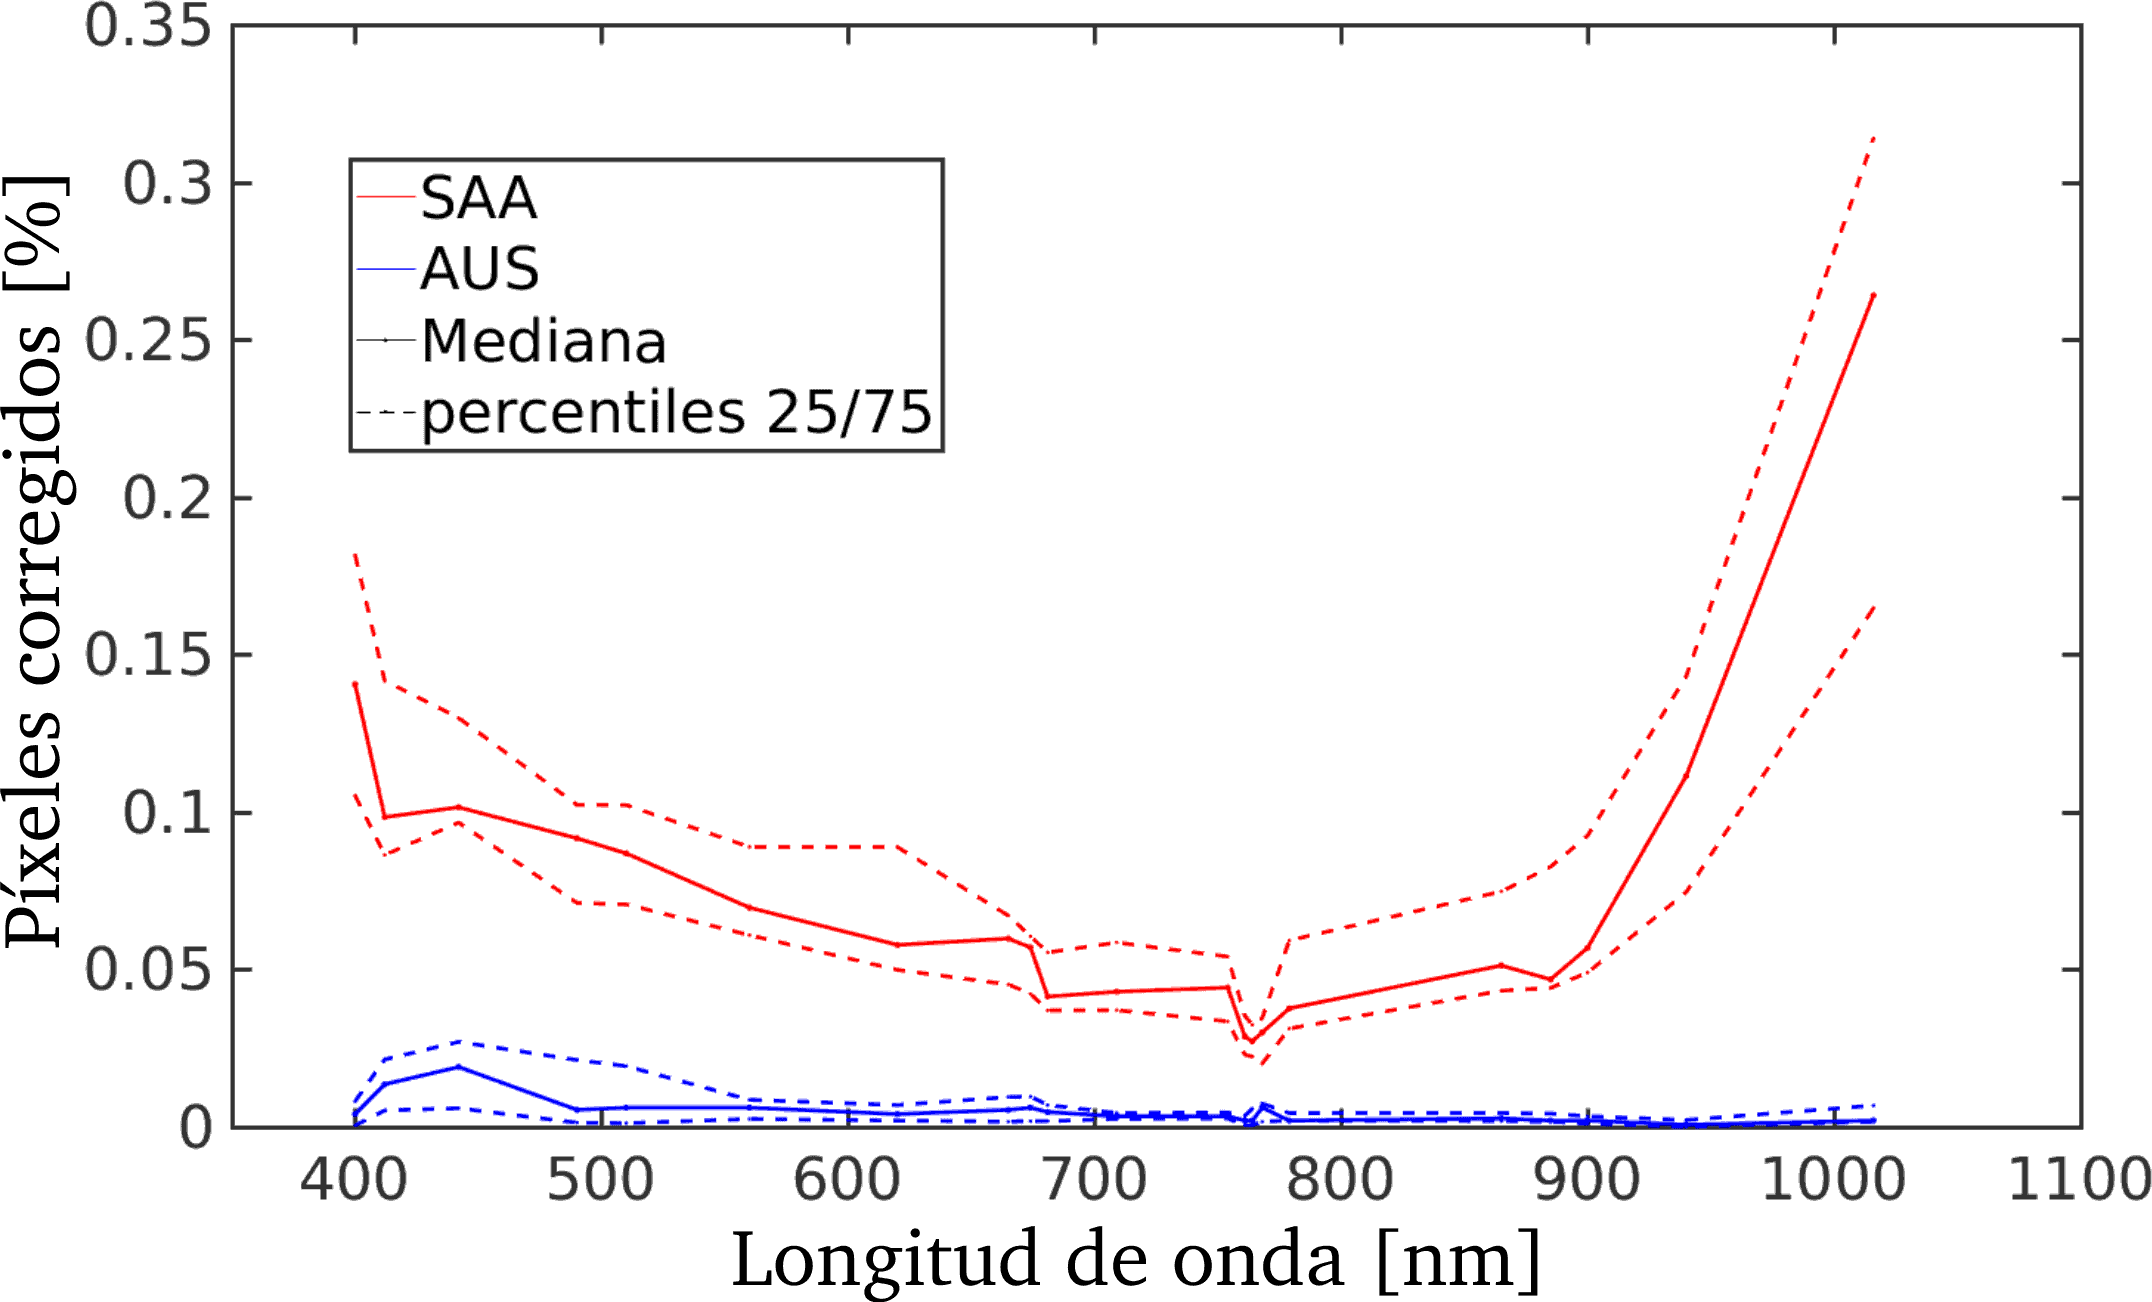
\includegraphics[width=0.8\textwidth]{ppe/figures/ppeBands}
    \caption[Porcentaje de píxeles marcados como contaminados con EPVs, calculados sobre prociones de imágenes en las regiones SAA y AUS.]{Porcentaje de píxeles marcados como contaminados con EPVs, evaluados en un conjunto de 18 subconjuntos de $1 \degree \times 1 \degree$, 9 de cada región, SAA (curvas rojas) y AUS (curvas azules). La cantidad de píxeles afectados es en promedio 27.8 veces mayor en la región SAA, aunque la diferencia es mayor en los extremos espectrales (bandas Oa\_01 [400 nm] y Oa\_21 [1016 nm]).}
    \label{ppe:ppeBands}
    \end{figure}
    
    Otra cantidad interesante para analizar es la corrección absoluta aplicada sobre los píxeles marcados con EPVs, es decir, la distribución de $|L^{TOA}_{r,c}-mdn(L^{TOA}_{r',c})|$, dado que un píxel fue marcado como afectado por un EPV (véase Ec. \ref{ppe:eq:ppr}). La Fig. \ref{ppe:ppeHists} muestra los histogramas normalizados de $|L^{TOA}_{r,c}-mdn(L^{TOA}_{r',c})|$ para píxeles marcados con EPV (etiquetado como error en la radiancia a TOA) para las bandas de 400 nm (a), 681 nm (b), 754 nm (c) y 1016 nm (d). En todos los casos, los histogramas se asemejan al decaimiento exponencial desplazado predicho por D' Amico et al. 2015 (Figura 6.3.2 \cite{damico2015}).


    \begin{figure}
    \centering
    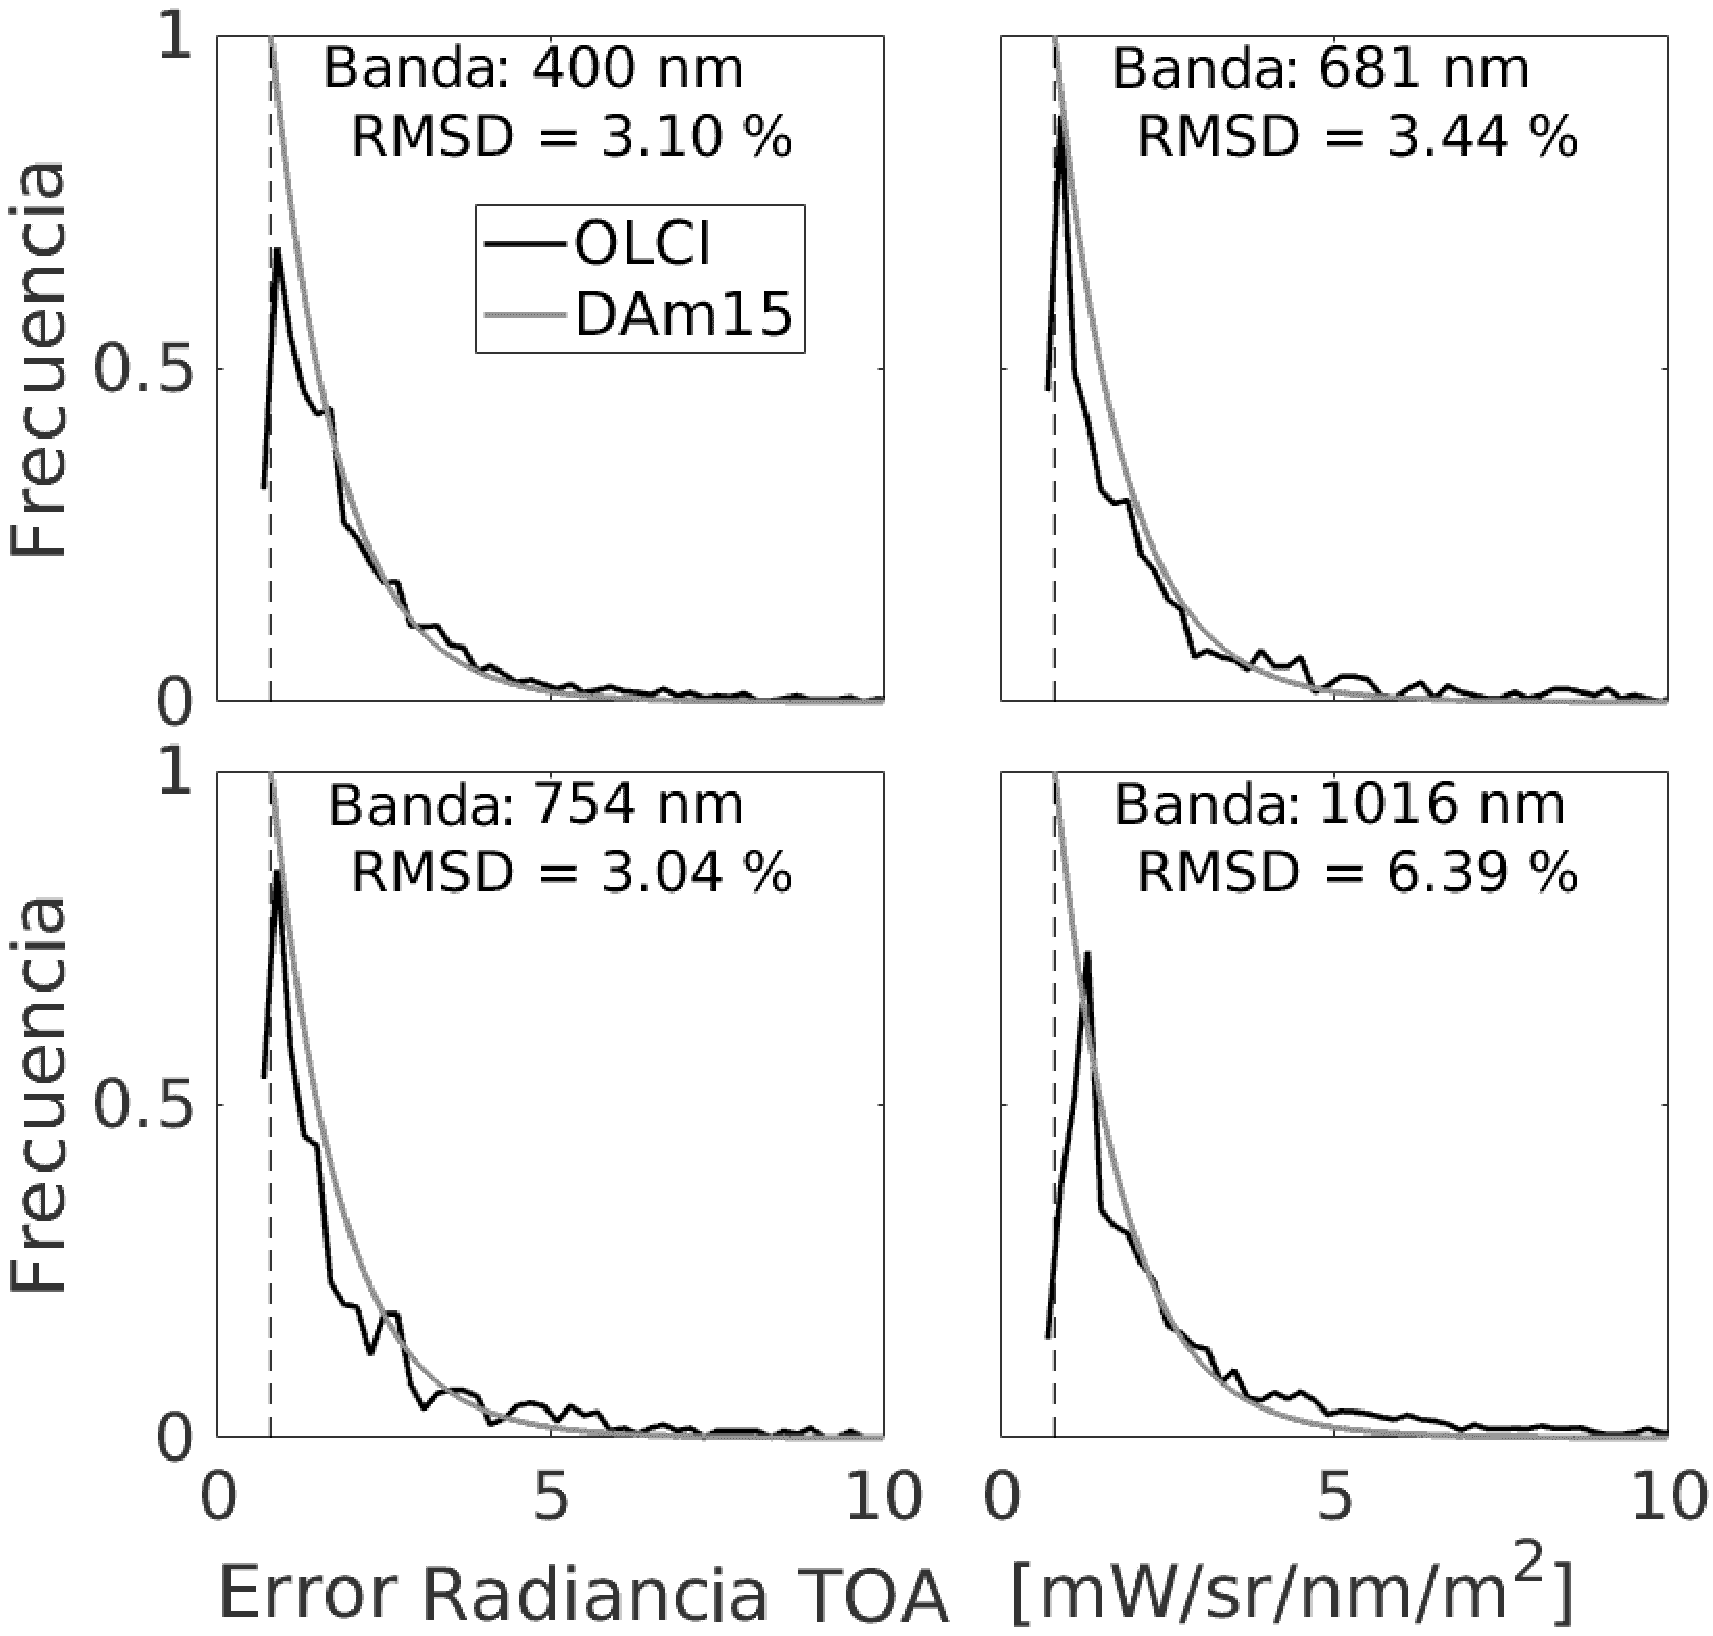
\includegraphics[width=0.5\textwidth]{ppe/figures/ppeHists}
    \caption[Distribución de probabilidad condicional del error absoluto en la radiancia a TOA, dada la detección de un EPV.]{Distribución de probabilidad condicional del error absoluto en la radiancia a TOA, dada la detección de un EPV, $p(| L^{TOA}_{r,c}-mdn(L^{TOA}_{r',c})| |EPV) $, para las bandas 400 (a), 681 (b), 709 (c) y 1016 nm (d). En negro, los valores obtenidos sobre las imágenes OLCI del subconjunto SAA aplicando el algoritmo EPV. En gris claro, distribución prevista por D' Amico et al. 2015 \cite{damico2015}, junto con una línea vertical punteada a 0.81 $mW/nm/sr/m^{2}$, indicando el error mínimo esperado.}
    \label{ppe:ppeHists}
    \end{figure}

    Como ejemplo de cómo los EPVs pueden afectar el desempeño de determinado producto biogeofísico, la Fig. \ref{ppe:ppeMci} muestra un mapa de Índice de Clorofila Máxima, calculada usando la Ec. \ref{ppe:eq:mci}. Gower et al. 2008, \cite{gower2008b}, ya comprobaron que se producían una gran cantidad de falsas alarmas de MCI aisladas en la región afectada por la SAA, y atribuyeron este fenómeno a los EPVs. Lo que se muestra en la Fig. \ref{ppe:ppeMci} respalda claramente esta afirmación, dado que en la imagen sin corregir (Fig. \ref{ppe:ppeMci}b) se observan franjas transversales aisladas de valores MCI extremadamente bajos/altos (hasta 15 $mW/nm/sr/m^{2}$ en los peores casos) probablemente no debidos a causas de origen oceanográfico. Después del esquema de eliminación de EPVs, estos valores extremos aislados tienden a suavizarse, como se muestra en la Fig.\ref{ppe:ppeMci}c. Este mismo comportamiento se observa en todo el conjunto de imágenes seleccionadas en la región SAA.

    \begin{figure*}
    \centering
    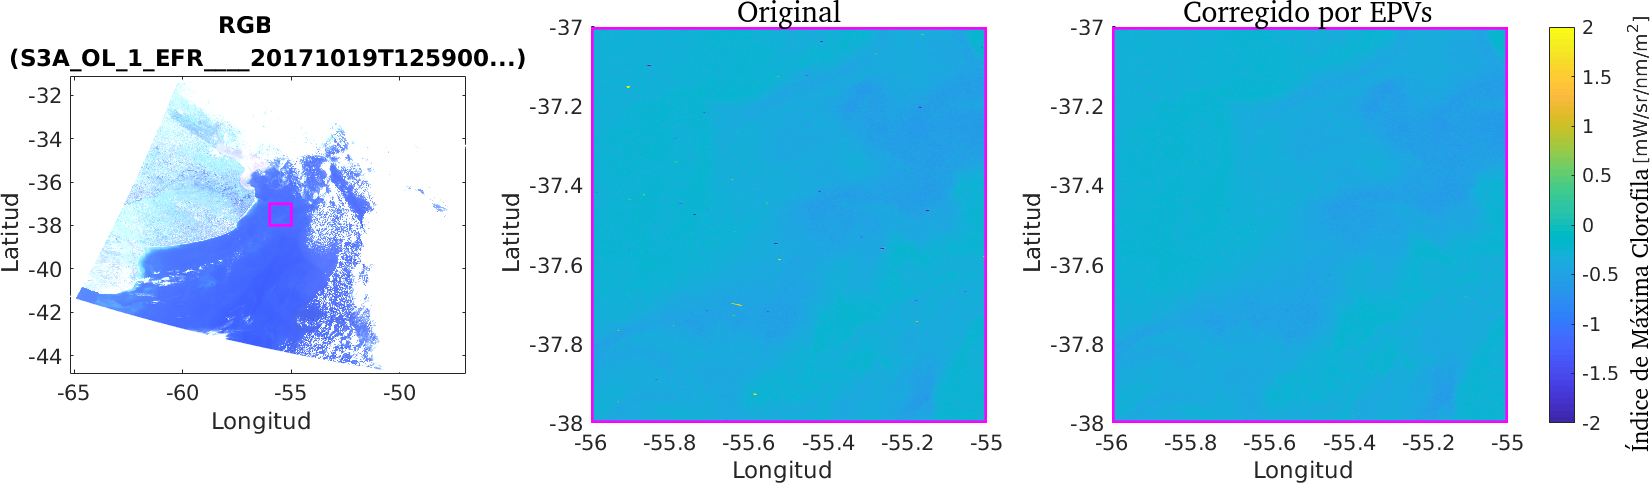
\includegraphics[width=0.9\textwidth]{ppe/figures/ppeMci}
    \caption[Reducción de las falsas alarmas sobre MCI al aplicar el algoritmo de eliminación de EPVs propuesto en este estudio.]{Reducción de las falsas alarmas sobre el Índice de Clorofila Máxima (MCI) al aplicar el algoritmo de eliminación de EPVs propuesto en este estudio. a) Composición RGB de imagen del conjunto SAA (2017-10-19T12:59:00Z), correspondiente al Mar Argentino. b) MCI calculado en un subconjunto de $1\degree \times 1\degree$ (utilizando la Ec. \ref{ppe:eq:mci}), donde el impacto de los EPV es fácilmente reconocible como valores de MCI extremadamente bajos/altos en franjas de píxeles aisladas, ortogonales a la dirección de barrido c) Igual que b) pero luego de la eliminación de los EPVs.}
    \label{ppe:ppeMci}
    \end{figure*}

\section{Conclusiones}
\label{ppe:s:conclusion}

    En el presente capítulo se propuso e implementó un esquema para la detección y eliminación de Eventos de Partículas Veloces (EPVs) de las imágenes de color del mar nivel L1B de OLCI. Se basa en un método píxel a píxel que consiste en aplicar un núcleo de 5 px $\times$ 1 px orientado \textit{along-track} y que se aplica a todas las bandas. Como se predijo, se observó que los EPVs afectan en promedio 27.8 veces más píxeles dentro de la Anomalía Magnética del Atlántico Sur que en otras regiones geográficas. Los errores absolutos en las radiancias a tope de la atmósfera inducidas por los EPVs siguen un patrón similar al predicho por D' Amico et al. 2015, \cite{damico2015}, es decir, una función de densidad de probabilidad de decaimiento exponencial desplazada, de escala característica de 1 y sesgo inicial de 0.81 $mW/nm/sr/m^{2}$ \cite{damico2015}. Como ejemplo de cómo los EPVs pueden inducir una falla en el desempeño de los productos biogeofísicos, Gower et al. 2008 alertó sobre la presencia de alarmas aisladas anómalas en el cómputo del Índice de Máxima Clorofila, especialmente en la región SAA \cite{gower2008b}. Se muestra cómo estas falsas alarmas aisladas se reducirán notablemente aplicando el esquema de eliminación de EPVs sobre imágenes L1B.
    A pesar de que los EPVs son altamente improbables fuera de la región SAA, la probabilidad de ocurrencia no se reduce a cero. Teniendo esto en cuenta y el hecho de que el campo geomagnético no es estacionario, se recomienda aplicar el esquema de eliminación de EPVs descrito sobre todas las imágenes L1B, y no sólo sobre la región del Atlántico Sur. El algoritmo propuesto se puede extender fácilmente a otros sensores sensibles al impacto de EPVs que vuelan en órbitas terrestres bajas (LEOs).  En \href{https://github.com/juanchossn/scripts_tesis_doctoral}{\textbf{\underline{este repositorio}}}\cite{repo} se podrán hallar los principales \textit{scripts} utilizados para implementar el esquema de detección de EPVs sobre imágenes OLCI L1B.